\documentclass[10pt,aspectratio=169]{beamer}
% compile: pdflatex presentation_en.tex  (twice from inside docs/)
% or push to GitHub -- .github/workflows/ auto-compiles

\usepackage[utf8]{inputenc}
\usepackage[T1]{fontenc}
\usepackage{lmodern}
\usepackage{amsmath}
\usepackage{amssymb}
\usepackage{booktabs}
\usepackage{array}
\usepackage{graphicx}
\usepackage{grffile}
\usepackage{xcolor}
\usepackage{tikz}
\usetikzlibrary{arrows.meta,shapes,positioning,calc}

\usetheme{Berlin}
\usecolortheme{seahorse}
\setbeamertemplate{footline}[frame number]
\setbeamertemplate{navigation symbols}{}

\newcommand{\bk}{\hfill\hyperlink{toc}{\beamerreturnbutton{Agenda}}}
\newcommand{\miplink}{\hyperlink{mip1}{\beamergotobutton{Full MIP (appendix)}}}

\title{\large Elective Surgery Scheduling}
\subtitle{Interval-based CP-SAT model for weekly OR planning}
\author{Hector Bonilla}
\date{}

\begin{document}

% ============================================================
\begin{frame}\titlepage\end{frame}

\begin{frame}{Agenda}
  \hypertarget{toc}{}
  \tableofcontents
  \vspace{0.4em}
  \footnotesize 20-minute flow: problem context and Portuguese case study
  $\to$ CP-SAT formulation $\to$ experimental results $\to$ conclusions.
  The MIP comparison model, full variable reference, pipeline diagram,
  and deployment notes are in the appendix.
\end{frame}

% ============================================================
\section{Problem \& Case Study}

\begin{frame}{The scheduling problem}
  \textbf{One hospital, one week. An elective waiting list always bigger
  than the week's OR capacity.}
  \begin{itemize}\small
    \item \textbf{Decision per case:} which room, which day, what start
      time, which surgeon -- or defer to next week.
    \item \textbf{Feasibility:} rooms, surgeons, shared equipment, and
      downstream recovery beds are all finite and shared.
    \item \textbf{Fairness:} clinical urgency, not FIFO order, should
      determine priority -- an overdue patient must not wait behind a
      routine one indefinitely.
    \item \textbf{Cost:} OR time runs $\sim\$30$--$40$/min once staffing
      and overhead are amortised (Macario, 2010). An idle minute today
      cannot be banked for tomorrow.
    \item \textbf{Scope:} \emph{advance scheduling} -- assigning cases
      to days and rooms before the week starts (Cardoen et al., 2010) --
      distinct from same-day sequencing or emergency disruption handling.
  \end{itemize}
\end{frame}

\begin{frame}{Case study: Portugal's SIGIC system}
  \textbf{SIGIC} (\emph{Sistema Integrado de Gest\~ao de Inscritos para
  Cirurgia}) -- Portugal's national elective surgical waiting-list
  management system, established by \textbf{Portaria n.\textsuperscript{o}
  45/2008} (Di\'ario da Rep\'ublica).

  \vspace{0.4em}
  Every elective case is assigned one of \textbf{four clinical priority
  tiers}, each with a legislated \textbf{maximum acceptable wait}:

  \vspace{0.3em}
  \begin{center}\small
  \begin{tabular}{clcc}
    \toprule
    Priority & Clinical meaning & Max wait & Model parameter \\
    \midrule
    1 & Routine elective & 270 days & $\text{wl}^{max}_1 = 270$ \\
    2 & Elevated urgency & 60 days  & $\text{wl}^{max}_2 = 60$  \\
    3 & Urgent           & 15 days  & $\text{wl}^{max}_3 = 15$  \\
    4 & Emergent add-on (run this week) & 3 days & $\text{wl}^{max}_4 = 3$ \\
    \bottomrule
  \end{tabular}
  \end{center}
  \vspace{0.3em}
  \footnotesize These four numbers are the model's $\text{wl}^{max}_p$
  parameters -- taken directly from a real, legislated, annually audited
  policy. The same tier structure appears in the UK NHS RTT targets and
  Canadian provincial wait-time benchmarks.
\end{frame}

\begin{frame}{Case study: the 2016 CHLN audit}
  Marques \& Captivo (2015) audited the \textbf{Centro Hospitalar Lisboa
  Norte (CHLN)} waiting list against SIGIC targets:
  \begin{itemize}\small
    \item $\sim$\textbf{7{,}400} patients on the waiting list at audit time.
    \item \textbf{16\%} had \emph{already} breached their tier's maximum-wait
      deadline.
    \item Average overrun among breached cases: \textbf{147 days}
      hospital-wide.
    \item Worst service -- Neurosurgery: $\sim$\textbf{261 days} average
      overrun among its breached patients.
  \end{itemize}
  \pause
  \begin{block}{Why these numbers shape this model's objective}
    A planner maximising throughput alone can report excellent utilisation
    while quietly reproducing this failure: scheduling routine cases,
    deferring overdue ones indefinitely, because a FIFO queue or an
    unweighted objective cannot distinguish them.
    The \textbf{non-scheduling penalty $w_c$} exists specifically to make
    breach costs \emph{explicit, priority-weighted, and dominant} in the
    objective -- so the optimiser cannot accidentally reproduce the audit
    finding.
  \end{block}
\end{frame}

% ============================================================
\section{CP-SAT Model}

\begin{frame}{What the model covers -- and what it doesn't}
  \begin{columns}
    \begin{column}{0.48\textwidth}
      \textbf{Modelled:}
      \begin{itemize}\footnotesize
        \item Case $\to$ room $\to$ time $\to$ surgeon assignment
        \item Room / service rosters (block schedule)
        \item Surgeon availability, daily and weekly limits
        \item One shared imaging unit (C-arm) with capacity
        \item Recovery / ICU bed pool (multi-day stay)
        \item Priority-4 emergency hard lock to day 1
        \item Paediatric-block carve-out rule
      \end{itemize}
    \end{column}
    \begin{column}{0.48\textwidth}
      \textbf{Deliberately excluded:}
      \begin{itemize}\footnotesize
        \item Stochastic durations
        \item Same-day disruptions / emergency adds
        \item Nurse / anaesthetist rostering
        \item Sequence-dependent OR cleaning
        \item Multi-week rolling horizon
        \item Emergency capacity reserve sizing
      \end{itemize}
    \end{column}
  \end{columns}
  \vspace{0.5em}
  \textbf{Key assumptions (full justification: FORMULATION.md \S2):}
  \begin{itemize}\footnotesize
    \item Deterministic durations (historical median per procedure).
    \item Turnover bucketed by case duration: 15 / 25 / 40 min.
    \item Surgeons as the binding staffing resource (nurses assumed
      bundled with the rostered room).
    \item Constant bed capacity across the week; explicit overflow charge
      for stays crossing the horizon.
  \end{itemize}
\end{frame}

\begin{frame}{Why CP-SAT and not a MIP?}
  \begin{block}{Core argument -- counting $\neq$ non-overlap for shared
  resources}
    ``Total equipment-use minutes today $\le$ capacity'' certifies that
    durations \emph{fit}. It does \emph{not} certify they don't
    \emph{collide in time}. For a single room these coincide; for a
    resource shared across multiple rooms they stop coinciding.
  \end{block}
  \vspace{0.2em}
  \begin{columns}
    \begin{column}{0.48\textwidth}\footnotesize
      \textbf{MIP (day-bucket):} count C-arm uses per day $\le1$.
      Two non-overlapping C-arm cases on the same day \emph{fail} this
      check even if they never run concurrently
      $\Rightarrow$ feasible schedules are forbidden.
    \end{column}
    \begin{column}{0.48\textwidth}\footnotesize
      \textbf{CP-SAT:} \texttt{AddCumulative} checks literal time
      overlap. Two sequential C-arm cases pass if they never run
      concurrently $\Rightarrow$ larger, correct feasible region
      $\Rightarrow$ strictly better schedules.
    \end{column}
  \end{columns}
  \vspace{0.4em}
  \textbf{Structural reason -- C11 (recovery/ICU beds):} the constraint
  ``$\text{bed}_c$ starts on the day $c$ is operated'' requires a
  variable holding ``day of surgery'' as a concrete \emph{value}.
  A day-bucket MIP has no such variable -- C11 cannot be expressed in
  that formulation at all, regardless of solver performance.
  \miplink
\end{frame}

\begin{frame}{Sets and parameters}
  \begin{columns}
    \begin{column}{0.44\textwidth}
      \textbf{Sets and indices}\vspace{0.2em}
      \begin{center}\footnotesize
      \begin{tabular}{cl}
        \toprule
        Symbol & Meaning \\
        \midrule
        $c\in C$ & Surgical cases \\
        $d\in D$ & Days $\{1,\dots,5\}$ \\
        $r\in R$ & Operating rooms \\
        $h\in H$ & Surgeons \\
        $e\in E$ & Shared equipment types \\
        $D_c\subseteq D$ & Eligible days for $c$ \\
        \bottomrule
      \end{tabular}
      \end{center}
    \end{column}
    \begin{column}{0.54\textwidth}
      \textbf{Key parameters}\vspace{0.2em}
      \begin{center}\footnotesize
      \begin{tabular}{cl}
        \toprule
        Symbol & Meaning \\
        \midrule
        $t_c^{op},t_c^{clean},t_c^{tot}$ & Duration, turnover, total \\
        $k_{dr}$, $k_{hd}$, $k_h$ & Room / surgeon daily / weekly cap \\
        $p_c\in\{1..4\}$ & Priority tier (SIGIC) \\
        $\text{wl}_c$ & Days waited at planning date \\
        $\text{wl}^{max}_p$ & Max wait for tier $p$: 270/60/15/3 \\
        $dd_c = \text{wl}^{max}_{p_c}-\text{wl}_c$ & Slack ($<0$ = overdue) \\
        $\mu_p = \text{wl}^{max}_1/\text{wl}^{max}_p$ & Priority multiplier \\
        $\alpha>1$ & Urgency amplifier for overdue cases \\
        $u_{ce},\kappa_{ed}$ & Equipment need, daily capacity \\
        $\rho(c),\text{los}_c,\beta_\rho$ & Bed pool, stay, capacity \\
        $\pi^{ovf}$ & Bed-overflow charge per day \\
        \bottomrule
      \end{tabular}
      \end{center}
    \end{column}
  \end{columns}
  \vspace{0.3em}
  \footnotesize\textbf{Priority multipliers derived from SIGIC:}
  $\mu_2=270/60=4.5$,\; $\mu_3=270/15=18$,\; $\mu_4=270/3=90$.
  A tier whose policy allows only $1/18$ of P1's wait is, by that same
  policy, $18\times$ more wait-sensitive.
\end{frame}

\begin{frame}{Decision variables}
  \textbf{Presence and scheduling} -- for every eligible $(c,d,r)$:
  \[\small
    \text{pr}_{cdr}\in\{0,1\},\quad
    \text{start}_{cdr},\;\text{end}_{cdr}\in[0,k_{dr}]
  \]
  For every non-priority-4 case: $u_c\in\{0,1\}$,\quad
  $\sum_{d,r}\text{pr}_{cdr}+u_c=1$

  \vspace{0.3em}
  \textbf{Two interval variables per candidate -- the key design choice:}
  \[\small
    \text{iv}_{cdr}=\texttt{NewOptionalIntervalVar}(\text{start},\;t_c^{tot},\;\text{end},\;\text{pr}_{cdr})
    \quad\textbf{[ROOM]}
  \]
  \[\small
    \text{sgiv}_{cdr}=\texttt{NewOptionalIntervalVar}(\text{start},\;t_c^{op},\;\text{sgend},\;\text{pr}_{cdr})
    \quad\textbf{[SURGEON]}
  \]
  \begin{block}{Why two intervals?}
    \small Surgeon H operates Case X: $t^{op}=70$, $t^{clean}=20$, starts at
    $t=0$. The \emph{room} stays blocked until $t=90$. The \emph{surgeon}
    is free at $t=70$ and can scrub into Room 2 for Case Y while Room 1
    is cleaned. A single $t^{tot}$-sized interval for C8 would wrongly
    keep the surgeon blocked until $t=90$ in every room. Giving C7
    (room, size $t^{tot}$) and C8 (surgeon, size $t^{op}$) the same
    \texttt{start} resolves this without any extra channelling constraint.
  \end{block}
\end{frame}

\begin{frame}{Objective function}
  \[\small
    \min\;
    \underbrace{\sum_{\substack{c:\,dd_c\ge0\\d\in D_c,r}}
      [dd_c+d]\,\text{pr}_{cdr}}_{\text{Term 1 -- on-time, earlier preferred}}
    +\;
    \underbrace{\sum_{\substack{c:\,dd_c<0\\d\in D_c,r}}
      [dd_c+\alpha d]\,\text{pr}_{cdr}}_{\text{Term 2 -- overdue, front-loaded}}
    +\;
    \underbrace{\sum_{c:\,p_c\ne4} w_c\,u_c}_{\text{Term 3 -- non-scheduling penalty}}
    +\;
    \underbrace{\pi^{ovf}\!\!\sum_{c:\,\rho(c)\ne\text{none}}\!\!\text{overflow}_c}_{\text{Term 4 -- bed overflow}}
  \]
  \[\small
    w_c = \mu_{p_c}\cdot\text{PenaltyCurve}(dd_c) + 1.2\cdot\max_{c'\in C}dd_{c'}
  \]
  \begin{itemize}\footnotesize
    \item \textbf{Term 1:} schedules cases on-time, preferring earlier days.
    \item \textbf{Term 2:} for overdue cases, $\alpha>1$ makes the planner
      front-load them to limit further delay.
    \item \textbf{Term 3 (dominant):} $w_c$ is calibrated so the model
      \emph{always} prefers scheduling over dropping; penalty escalates
      sharply past the SIGIC deadline and with higher priority.
    \item \textbf{Term 4:} makes bed-overflow cost explicit; forces the
      model to account for stays crossing the planning horizon.
  \end{itemize}
  \footnotesize\textbf{PenaltyCurve} (\texttt{src/model/penalty.py}): flat
  while the case has slack, escalates sharply on breach, keeps rising with
  backlog -- the shape that makes this objective reproduce SIGIC's intent.
\end{frame}

\begin{frame}{Constraints C1--C6: case disposition and eligibility}
  \textbf{C1 -- at most one occurrence per patient per week:}
  \[\small
    \sum_{c:\,\text{patient}(c)=n}\!\sum_{d\in D_c,r}\text{pr}_{cdr}\le1
    \qquad\forall n
  \]
  \textbf{C2 -- priority-4 cases locked to day 1:}
  \[\small
    \sum_r\text{pr}_{c,1,r}=1
    \qquad\forall c:\;p_c=4
    \quad\text{(all other slots forced to 0)}
  \]
  \textbf{C3 -- every other case is scheduled exactly once or penalised:}
  \[\small
    \sum_{d\in D_c,r}\text{pr}_{cdr}+u_c=1
    \qquad\forall c:\;p_c\ne4
  \]
  \textbf{C4--C6 -- eligibility (resolved at build time, never solver rows):}
  \begin{itemize}\footnotesize
    \item \textbf{C4:} room-service roster match (e.g.\ VASC cases only in VASC rooms).
    \item \textbf{C5:} ambulatory-only rooms reject cases requiring overnight stay.
    \item \textbf{C6:} paediatric-block rule -- Friday ENT rooms restricted to age $\le8$.
  \end{itemize}
  \footnotesize Eligibility runs once at candidate-generation time. No
  $\text{pr}_{cdr}$ is ever created for an ineligible $(c,d,r)$ triple --
  the main variable-count reduction, costing nothing at solve time.
\end{frame}

\begin{frame}{Constraints C7--C11: time, resources, and beds}
  \textbf{C7 -- room non-overlap (exact):}\quad
  $\texttt{AddNoOverlap}(\{\text{iv}_{cdr}:\;d,r\text{ fixed}\})\;\forall d,r$

  \smallskip
  \textbf{C8 -- surgeon non-overlap (on surgeon's own interval):}\quad
  $\texttt{AddNoOverlap}(\{\text{sgiv}_{cdr}:\;\text{surg}(c)=h,\;d\text{ fixed}\})\;\forall h,d$

  \smallskip
  \textbf{C9 -- surgeon capacity (daily and weekly):}
  \[\small
    \sum_{c:\,\text{surg}(c)=h}\!\sum_r t_c^{op}\,\text{pr}_{cdr}\le k_{hd}\;\forall h,d
    \qquad
    \sum_{c,d,r} t_c^{op}\,\text{pr}_{cdr}\le k_h\;\forall h
  \]

  \textbf{C10 -- shared equipment, exact time-overlap check:}\quad
  $\texttt{AddCumulative}(\{\text{iv}_{cdr}:\;u_{ce}=1,\;d\},\;\mathbf{1},\;\kappa_{ed})\;\forall e,d$

  \textbf{C11 -- recovery/ICU beds (multi-day, with horizon overflow):}
  \begin{itemize}\footnotesize
    \item $\text{dayof}_c\leftarrow d_\text{idx}$
      via \texttt{OnlyEnforceIf}($\text{pr}_{cdr}=1$).
    \item $\text{bed}_c=\texttt{NewOptionalIntervalVar}
      (\text{dayof}_c,\;\text{los}_c,\;\text{dayof}_c+\text{los}_c,\;1-u_c)$
    \item $\texttt{AddCumulative}(\{\text{bed}_c:\;\rho(c)=\rho\},\;\mathbf{1},\;\beta_\rho)
      \;\forall\rho$
    \item $\text{overflow}_c=\max(0,\;\text{dayof}_c+\text{los}_c-n_d)$
  \end{itemize}
  \footnotesize C10 is the ``correct C-arm'' constraint -- actual time
  overlap, not a day count. C11 requires a concrete ``day of surgery''
  value: structurally impossible in a day-bucket MIP.
\end{frame}

% ============================================================
\section{Data \& Results}

\begin{frame}{Test instances}
  \textbf{Demo instance -- 20 cases, 5 rooms, 6 surgeons, 3 services}
  \begin{center}\small
  \begin{tabular}{lccc}
    \toprule
    Service & Rooms & Capacity (min/day) & Surgeons \\
    \midrule
    ENT   & 2 & 360 ($\approx6$ h) & 2 \\
    ORTHO & 1 & 450 ($\approx7.5$ h) & 1 \\
    VASC  & 2 & 660 ($\approx11$ h) & 3 \\
    \bottomrule
  \end{tabular}
  \end{center}
  Activates \emph{every} constraint family in one run: 3 priority-4
  cases (C2), shared C-arm (C10), 2 ICU beds (C11), paediatric-block
  Friday rule (C6), 3 overdue cases already past their SIGIC deadline.

  \vspace{0.6em}
  \textbf{Medium instance -- 200 cases, 12 rooms, 17 surgeons, 5 services}
  \begin{itemize}\footnotesize
    \item VASC and NEURO share C-arm equipment; 12\% of cases need
      1--2 ICU days; priority mix 58/26/13/3\%.
    \item Used to measure the CP-vs-MIP performance gap at scale
      (Gurobi provides the true MIP optimum for comparison).
  \end{itemize}
\end{frame}

\begin{frame}{Demo instance: CP-SAT vs MIP -- results table}
  \texttt{\small python main.py --instance demo --benchmark --gap 0.0001}
  \begin{center}\small
  \begin{tabular}{lcccc}
    \toprule
    Solver & Status & Objective & Gap & Scheduled \\
    \midrule
    \textbf{CP-SAT (primary)} & Optimal & \textbf{155.0} & 0.00\% & 20/20 \\
    OR-Tools/CBC (MIP)        & Optimal & 157.0          & 0.00\% & 20/20 \\
    Gurobi (MIP)              & Optimal & 157.0          & 0.00\% & 20/20 \\
    CP Optimizer              & Optimal & 155.0          & 0.00\% & 20/20 \\
    \bottomrule
  \end{tabular}
  \end{center}
  \vspace{0.3em}
  \textbf{C-arm cases} (C14, C15, C17, C19 -- 4 VASC endovascular
  procedures):
  \begin{itemize}\small
    \item \textbf{CP-SAT:} Mon=[C19], Tue=[\textbf{C15, C17}], Wed=[C14]
      -- two C-arm cases placed on the \emph{same} day sequentially.
    \item \textbf{MIP:} Mon=[C19], Tue=[C15], Wed=[C17], Thu=[C14]
      -- one per day, forced by the day-count cap $\sum x_{cdr}\le1$.
  \end{itemize}
  \footnotesize Objective gap (155 vs.\ 157) comes entirely from this: CP-SAT
  correctly identifies that the two Tuesday C-arm cases never overlap in
  clock time, while the MIP's day-count constraint cannot detect that.
\end{frame}

\begin{frame}{Demo -- CP-SAT Gantt schedule}
  \begin{center}
    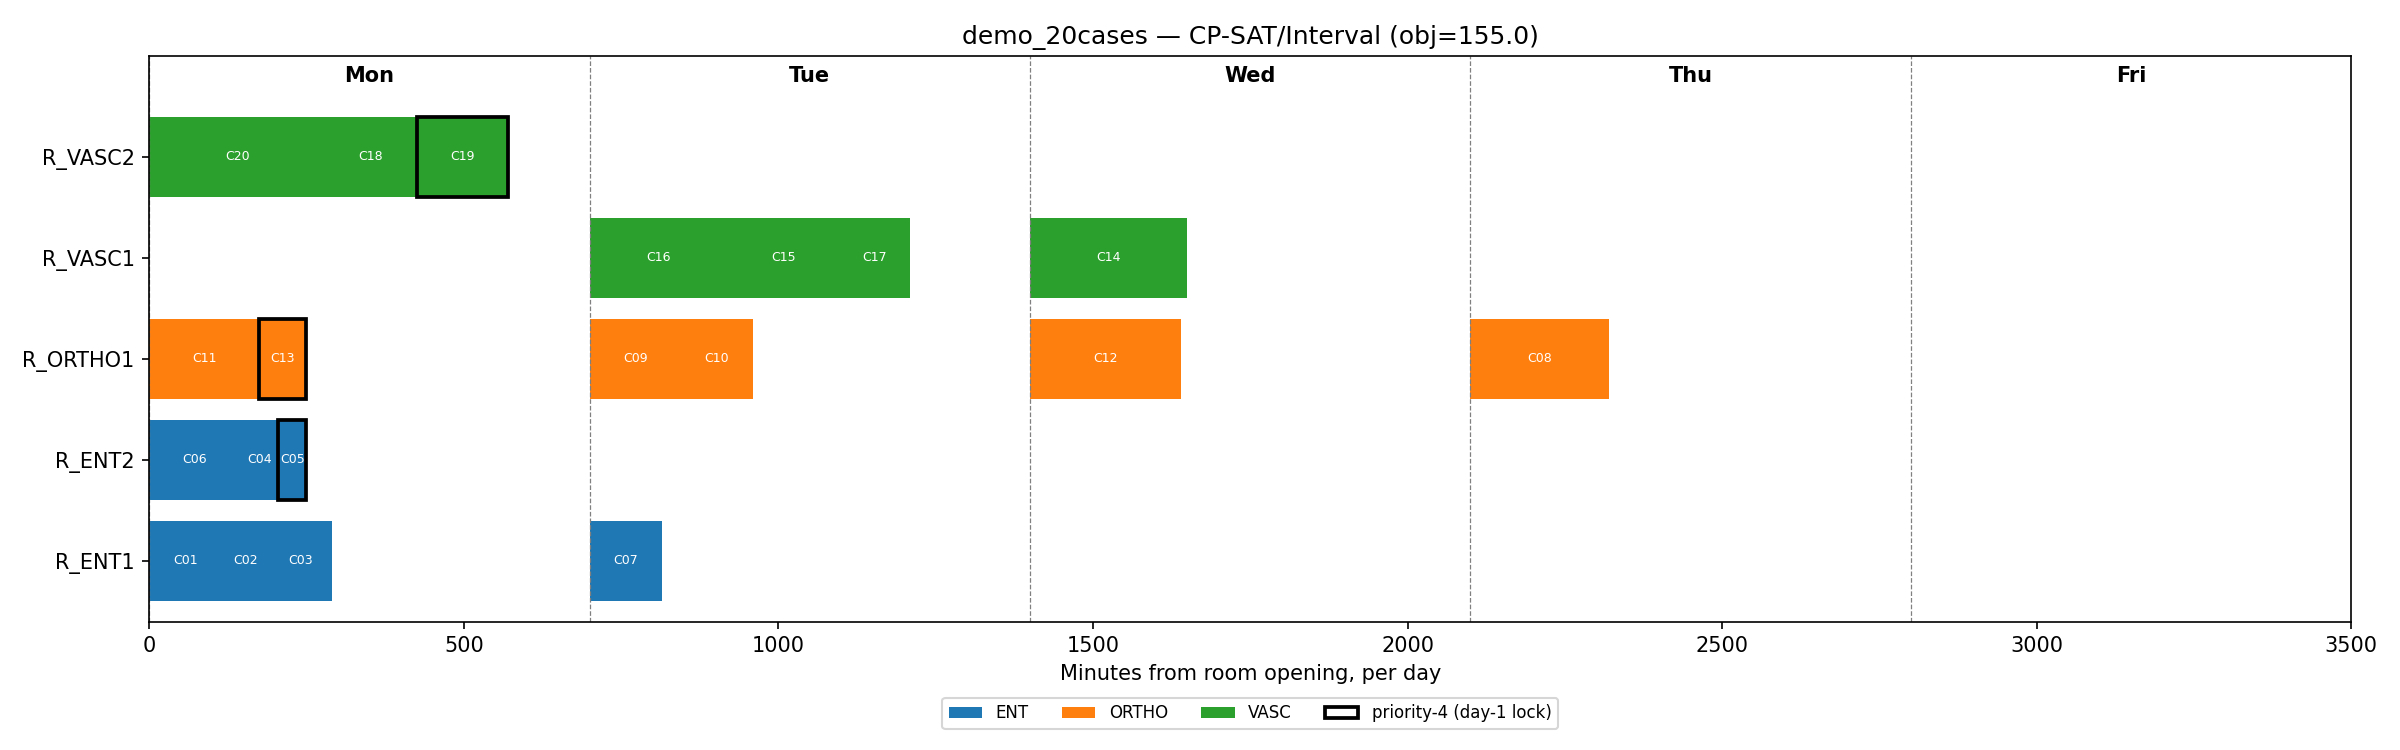
\includegraphics[width=0.96\linewidth]{img/demo_cp_sat.png}
  \end{center}
  \footnotesize\textbf{Reading the chart:} each row = one room; each bar = one
  case, coloured by service. Bold-outlined bars are priority-4 cases, all
  correctly placed on Monday.
  \textbf{Tuesday}: R\_VASC1 and R\_VASC2 each carry one C-arm case
  sequentially -- the model correctly places both on the same day because
  they never overlap in clock time.
\end{frame}

\begin{frame}{Demo -- MIP Gantt schedule (comparison)}
  \begin{center}
    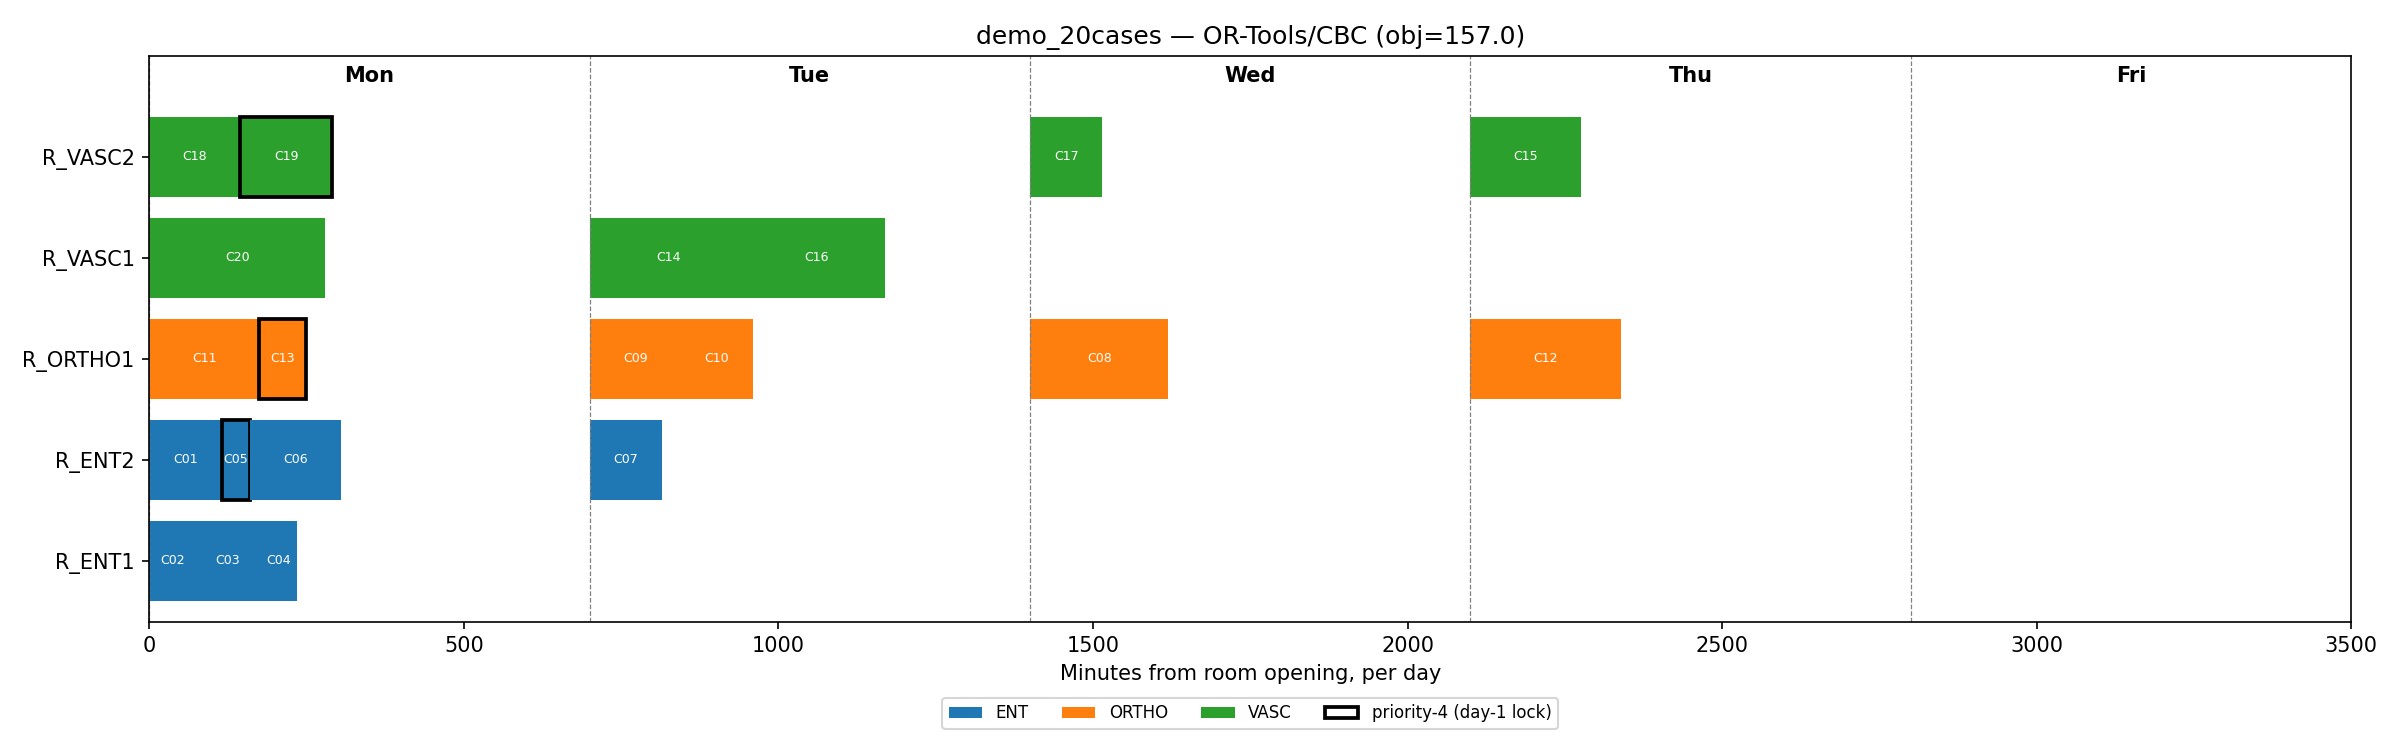
\includegraphics[width=0.96\linewidth]{img/demo_baseline_milp.png}
  \end{center}
  \footnotesize\textbf{Reading the chart:} same 20 cases, same services.
  The MIP produces no exact clock times (day-bucket formulation) -- bars
  are laid out back-to-back for display only; the solver makes no claim
  about their intra-day order.
  Compare C-arm spread: Mon, Tue, Wed, Thu each carry exactly one C-arm
  case. The day-count constraint $\sum x_{cdr}\le1$ is satisfied but it
  prohibits the more efficient two-in-a-day placement CP-SAT finds.
\end{frame}

\begin{frame}{Scaling up: medium instance (200 cases, 2-minute budget)}
  \textbf{Step 1 -- true MIP optimum} (Gurobi, near-zero gap):
  \textbf{74{,}074.0}, 130/200 scheduled, under 1 second.

  \textbf{Step 2 -- realistic 2-minute / 1\% gap budget:}
  \begin{center}\small
  \begin{tabular}{lcccc}
    \toprule
    Solver & Objective & Own gap & vs.\ true MIP opt. & Sched. \\
    \midrule
    Gurobi (reference) & 74{,}074.0 & 0.00\% & ---          & 130/200 \\
    OR-Tools/CBC       & 74{,}116.0 & 0.56\% & $+0.06\%$    & 130/200 \\
    \textbf{CP-SAT}    & \textbf{69{,}956.0} & 6.62\% & \textbf{$-5.56\%$} & \textbf{131/200} \\
    \bottomrule
  \end{tabular}
  \end{center}
  \vspace{0.3em}
  CBC reaches the MIP's own proven optimum. \textbf{CP-SAT beats that
  proven optimum by 5.56\%} while scheduling one additional case -- it
  searches a strictly larger, correct feasible region.

  \smallskip
  CP-SAT's own 6.62\% gap is measured against \emph{its own} larger
  feasible-region bound -- not evidence of poor search quality.
  The right comparison is the absolute objective value: \textbf{69{,}956
  vs. 74{,}074}.
\end{frame}

\begin{frame}{Medium instance -- CP-SAT Gantt (131 cases)}
  \begin{center}
    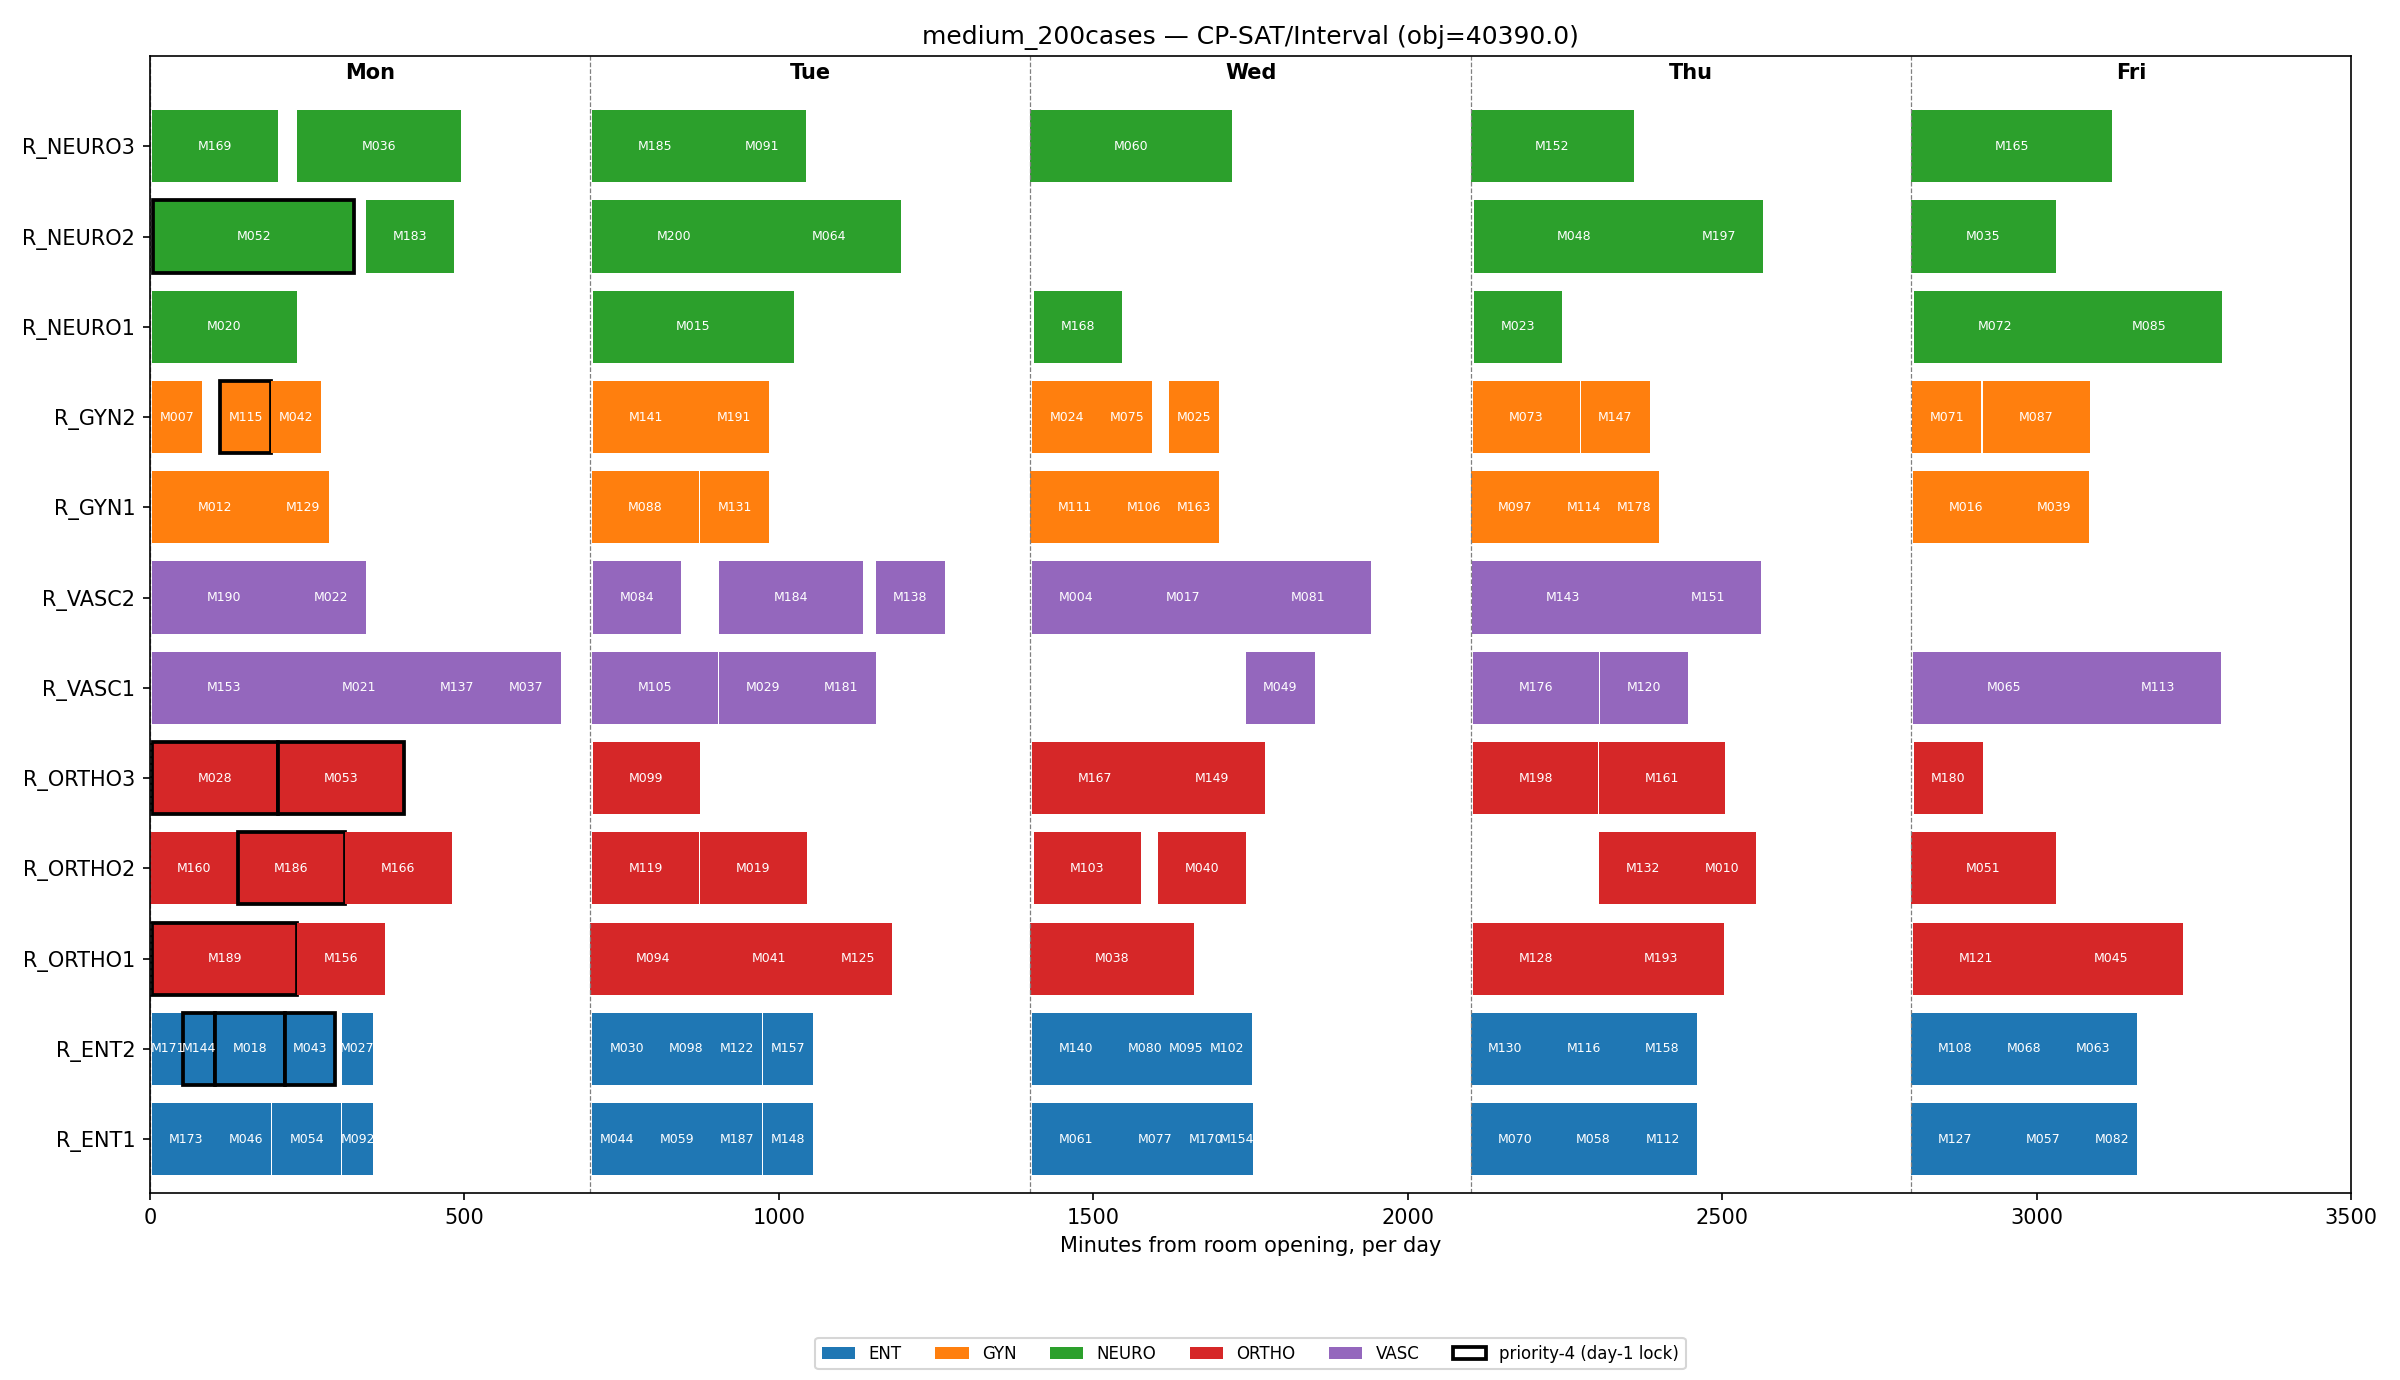
\includegraphics[width=0.96\linewidth]{img/medium_cp_sat.png}
  \end{center}
  \footnotesize\textbf{Reading the chart:} 12 rooms (rows), 5 days,
  131 scheduled cases with exact per-case start and end times.
  The schedule shows the model reasoning simultaneously over all five
  services, with C-ARM constraints active across the VASC and NEURO
  rooms. No two C-arm cases overlap in clock time on any day.
\end{frame}

% ============================================================
\section{Conclusions}

\begin{frame}{Conclusions}
  \begin{enumerate}\small
    \item \textbf{CP-SAT finds strictly better schedules on both instances.}
      Demo: 155.0 vs.\ 157.0 (MIP proven optimum). Medium: 69{,}956 vs.\
      74{,}074 (MIP's proven optimum) -- 5.56\% better, one more case
      scheduled. The cause is always the same: a larger, correct feasible
      region.
    \item \textbf{Gap percentages mislead without context.} CP-SAT's 6.62\%
      and CBC's 0.56\% are measured against \emph{different} feasible-region
      bounds. The correct comparison is absolute objective value -- CP-SAT
      wins by a wide margin.
    \item \textbf{Shared equipment modelling is the decisive structural factor.}
      \texttt{AddCumulative} checks actual clock-time overlap; the MIP's
      day-count cap incorrectly forbids non-overlapping same-day equipment
      uses.
    \item \textbf{C11 cannot be expressed in a day-bucket MIP.} No variable
      in that formulation holds ``day of surgery'' as a value -- a structural
      argument for interval-based CP, independent of performance.
    \item \textbf{The two-interval design reflects real OR practice.}
      A surgeon free at $t=70$ can move to a second room while Room 1 cleans
      until $t=90$ -- a single-interval model incorrectly forbids this.
    \item \textbf{Demo instance: proven optimal in $\sim$0.1~s.}
      Entirely practical for interactive decision support.
    \item \textbf{At a 2-minute budget, CP-SAT already dominates CBC} in
      both objective quality and cases scheduled.
  \end{enumerate}
\end{frame}

\begin{frame}{Questions}
  \centering\Large Thank you.
  \vspace{1em}
  \normalsize
  \hyperlink{toc}{\beamergotobutton{Back to agenda}}
  \quad
  \hyperlink{mip1}{\beamergotobutton{Full MIP appendix}}
\end{frame}

% ============================================================
\appendix
\section{Appendix}

\begin{frame}{CP-SAT variables -- complete formal reference}
  \tiny
  \begin{center}
  \begin{tabular}{p{3.0cm}p{2.9cm}p{6.4cm}}
    \toprule
    \textbf{Variable} & \textbf{Domain} & \textbf{Meaning} \\
    \midrule
    $\text{pr}_{cdr}$
      & $\{0,1\}$
      & 1 if case $c$ is scheduled day $d$ room $r$; created only for
        eligible $(c,d,r)$ triples (C4--C6 pre-filter) \\[2pt]
    $\text{start}_{cdr}$
      & $[0,k_{dr}]$
      & Start time (min from room opening) when $\text{pr}_{cdr}=1$ \\[2pt]
    $\text{end}_{cdr}$
      & $[0,k_{dr}]$
      & Room-block end $=\text{start}_{cdr}+t_c^{tot}$ \\[2pt]
    $\text{iv}_{cdr}$
      & \texttt{OptionalIntervalVar}
      & \textbf{Room} interval: $[\text{start},\,\text{start}+t_c^{tot})$;
        active iff $\text{pr}_{cdr}=1$; feeds C7, C10, C11 \\[2pt]
    $\text{sgend}_{cdr}$
      & $[0,k_{dr}]$
      & Surgeon-end $=\text{start}_{cdr}+t_c^{op}$ \\[2pt]
    $\text{sgiv}_{cdr}$
      & \texttt{OptionalIntervalVar}
      & \textbf{Surgeon} interval: $[\text{start},\,\text{start}+t_c^{op})$;
        active iff $\text{pr}_{cdr}=1$; feeds C8 only.
        Shorter than $\text{iv}_{cdr}$ by $t_c^{clean}$ \\[2pt]
    $u_c$
      & $\{0,1\}$
      & 1 if case $c$ is not scheduled (penalty $w_c$);
        only for $p_c\ne4$; enforced by C3 \\[2pt]
    $\text{dayof}_c$
      & $\{0,\dots,n_d-1\}$
      & Index of the day $c$ is scheduled on; derived via
        \texttt{OnlyEnforceIf} from $\text{pr}_{cdr}=1$;
        only built for cases with $\rho(c)\ne\text{none}$ \\[2pt]
    $\text{bed}_c$
      & \texttt{OptionalIntervalVar}
      & ICU/recovery interval: $[\text{dayof}_c,\,\text{dayof}_c+\text{los}_c)$;
        present iff $1-u_c=1$; feeds C11 Cumulative \\[2pt]
    $\text{overflow}_c$
      & $[0,\text{los}_c]$
      & Days of bed stay past the horizon;
        adds Term 4 to objective \\
    \bottomrule
  \end{tabular}
  \end{center}
  \bk
\end{frame}

\begin{frame}{CP-SAT search strategy}
  \begin{itemize}\small
    \item \textbf{Parallel portfolio:} several complete-search workers with
      different variable-ordering heuristics, plus Large Neighbourhood Search
      workers improving an incumbent, all sharing learned clauses via a
      common SAT core (Perron \& Furnon, Google OR-Tools).
    \item \textbf{No custom branching strategy:} OR-Tools' guidance is that
      the default portfolio outperforms hand-tuned single strategies unless
      you have structural insight not already exposed through
      \texttt{NoOverlap}/\texttt{Cumulative}. This model exposes that
      structure fully.
    \item \textbf{Workers} capped at \texttt{os.cpu\_count()} -- over-
      subscribing past physical cores adds thread contention, not search
      diversity.
    \item \textbf{Gap target} $=1\%$ by default; solver stops when the
      best bound is within 1\% of the current incumbent.
    \item \textbf{``Optimal'' means within the configured gap}, not a
      literal 0\% gap -- always printed and never assumed zero.
  \end{itemize}
  \bk
\end{frame}

\begin{frame}{CP-SAT integration pipeline}
  \centering
  % node width 1.75cm + gap 0.26cm  =>  5*1.75 + 4*0.26 = 9.79 cm total -- fits slide
  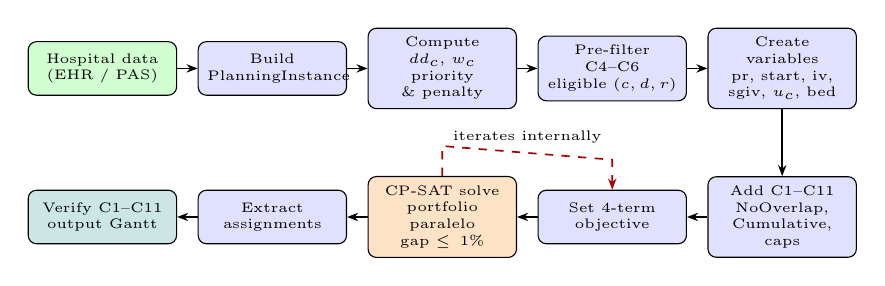
\begin{tikzpicture}[
    node distance=0.22cm and 0.26cm,
    base/.style={draw, rectangle, rounded corners=3pt,
                 align=center, font=\tiny,
                 minimum width=1.75cm, minimum height=0.68cm,
                 text width=1.65cm},
    proc/.style={base, fill=blue!12},
    ionode/.style={base, fill=green!18},
    solvenode/.style={base, fill=orange!22},
    outnode/.style={base, fill=teal!20},
    arr/.style={-{Stealth[length=4pt,width=3pt]}, semithick},
    backloop/.style={-{Stealth[length=4pt,width=3pt]}, semithick, dashed,
                     red!65!black},
  ]
    % ---- Row 1: left to right ----
    \node[ionode]  (A) {Hospital data\\(EHR / PAS)};
    \node[proc, right=of A] (B) {Build\\PlanningInstance};
    \node[proc, right=of B] (C) {Compute $dd_c$, $w_c$\\priority \& penalty};
    \node[proc, right=of C] (D) {Pre-filter C4--C6\\eligible $(c,d,r)$};
    \node[proc, right=of D] (E) {Create variables\\pr, start, iv,\\sgiv, $u_c$, bed};

    % ---- Row 2: right to left ----
    \node[proc,     below=0.85cm of E] (F) {Add C1--C11\\NoOverlap,\\Cumulative, caps};
    \node[proc,      left=of F]        (G) {Set 4-term\\objective};
    \node[solvenode, left=of G]        (H) {CP-SAT solve\\portfolio paralelo\\gap $\le1\%$};
    \node[proc,      left=of H]        (I) {Extract\\assignments};
    \node[outnode,   left=of I]        (J) {Verify C1--C11\\output Gantt};

    % ---- Row 1 arrows ----
    \draw[arr] (A)--(B); \draw[arr] (B)--(C);
    \draw[arr] (C)--(D); \draw[arr] (D)--(E);
    % ---- Connector between rows ----
    \draw[arr] (E)--(F);
    % ---- Row 2 arrows ----
    \draw[arr] (F)--(G); \draw[arr] (G)--(H);
    \draw[arr] (H)--(I); \draw[arr] (I)--(J);
    % ---- Re-solve loop (H -> G) using calc ----
    \draw[backloop]
      (H.north) -- ($(H.north)+(0,0.38)$)
      -- node[above,font=\tiny,text=black]{iterates internally}
      ($(G.north)+(0,0.38)$) -- (G.north);
  \end{tikzpicture}
  \vspace{0.3em}
  \footnotesize Each box maps to a file in the repo.
  The pre-filter (C4--C6) runs once at build time.
  The parallel portfolio runs $\le$\texttt{cpu\_count()} workers,
  each sharing learned clauses with the others.
  \bk
\end{frame}

\begin{frame}{When would MILP be the right choice?}
  \small Even within this problem class, MILP is the more natural choice in
  specific situations:
  \begin{itemize}
    \item \textbf{Day-assignment only, no clock times needed.} When the
      deliverable is ``case $c$ runs on day $d$ in room $r$'' without an
      exact start time, the day-bucket MIP naturally captures this.
    \item \textbf{No shared resources across rooms.} If each piece of
      equipment is dedicated to one room and surgeons do not move between
      rooms, the day-count constraint is sufficient.
    \item \textbf{No multi-day downstream constraint (C11).} When recovery
      beds are not modelled, one key structural reason for intervals
      disappears.
    \item \textbf{Small instance, LP relaxation is tight.} A commercial
      solver (Gurobi, CPLEX) can close the MIP gap in seconds with a
      provably optimal LP certificate -- faster than CP-SAT on small instances.
    \item \textbf{Need LP dual variables.} Shadow prices support sensitivity
      analysis and what-if reporting -- CP-SAT does not expose these.
    \item \textbf{Team expertise is in MILP.} Modelling risk of incorrectly
      encoding constraints is lower with the tool the team knows best.
  \end{itemize}
  \bk
\end{frame}

\begin{frame}{MIP -- formulation overview}
  \hypertarget{mip1}{}
  Implemented in \texttt{milp\_baseline\_solver.py}; runs via
  \texttt{--solver milp-cbc} (bundled), \texttt{milp-gurobi}, or
  \texttt{milp-cplex} (commercial license required).

  \textbf{Same as CP-SAT:} sets, eligibility pre-filter (C4--C6),
  priority tiers, $w_c$ from the same \texttt{penalty.py}.

  \textbf{Key differences:}
  \begin{itemize}\small
    \item No intra-day clock times -- decisions at day+room granularity only.
    \item C7 and C10 are linear capacity sums, not exact time-overlap checks.
    \item C11 (recovery beds) is \emph{not expressible} -- a day-bucket
      variable holds no ``day of surgery'' value for a multi-day stay.
    \item No Term 4 in the objective (C11 does not exist in this model).
  \end{itemize}
  \bk
\end{frame}

\begin{frame}{MIP -- variables}
  \footnotesize
  \begin{center}
  \begin{tabular}{p{2.4cm}p{2.6cm}p{6.6cm}}
    \toprule
    \textbf{Variable} & \textbf{Domain} & \textbf{Meaning} \\
    \midrule
    $x_{cdr}$ & $\{0,1\}$ &
      1 if case $c$ is scheduled on day $d$ in room $r$.
      Only created for eligible $(c,d,r)$ triples.
      Determines day and room but \emph{not} exact clock time. \\[3pt]
    $z_c$ & $[0,1]$ &
      1 if case $c$ is not scheduled this week (non-priority-4 only).
      Declared continuous -- C3 forces it to $\{0,1\}$ at the optimum
      because the objective penalises fractional non-scheduling. \\
    \bottomrule
  \end{tabular}
  \end{center}
  \vspace{0.3em}
  \textbf{Objective} (same three-term structure as CP-SAT, no Term 4):
  \[\footnotesize
    \min\;\sum_{c:\,dd_c\ge0}\sum_{d,r}[dd_c+d]\,x_{cdr}
    +\sum_{c:\,dd_c<0}\sum_{d,r}[dd_c+\alpha d]\,x_{cdr}
    +\sum_{c:\,p_c\ne4}w_c\,z_c
  \]
  \bk
\end{frame}

\begin{frame}{MIP -- constraints and what's missing}
  \textbf{C7 (room, aggregate sum):}
  \[\small
    \sum_{c\in C}t_c^{tot}\,x_{cdr}\le k_{dr}\qquad\forall d,r
  \]
  For a single room: equivalent to non-overlap. For a \emph{shared resource
  across rooms}: incorrectly treats all equipment-uses as simultaneous.

  \textbf{C10 (equipment, daily headcount):}
  \[\small
    \sum_{c:\,u_{ce}=1}\sum_r x_{cdr}\le\kappa_{ed}\qquad\forall e,d
  \]
  Counts \emph{how many} equipment-$e$ cases land on a day, not whether
  they overlap -- the main source of the 5.56\% objective gap vs.\ CP-SAT.

  \textbf{No C11:} ``$\text{bed}_c$ starts on whichever day $c$ is
  scheduled'' cannot be written -- no variable in a day-bucket model
  holds ``day of surgery'' as a \emph{value}.
  \bk
\end{frame}

\begin{frame}{CP Optimizer (optional, appendix)}
  \small Kept for one reason: \textbf{sequence-dependent room turnover}
  -- a per-adjacent-pair transition matrix via
  \texttt{sequence\_var + no\_overlap(transition\_matrix)}.
  \begin{center}\small
  \begin{tabular}{lcc}
    \toprule
    & Same service & Different service \\
    \midrule
    CP-SAT (duration-bucketed) & case's own $t_c^{clean}$ & same \\
    CP Optimizer & 15 min & 35 min \\
    \bottomrule
  \end{tabular}
  \end{center}
  Demo instance: identical to CP-SAT (155.0, 20/20, Optimal).

  At 200 cases, own gap closes slower than CP-SAT (search-tuning
  difference, no warm start applied -- not a modelling weakness).
  \bk
\end{frame}

\begin{frame}{Production deployment}
  \begin{enumerate}\small
    \item \textbf{Data loader:} map hospital EHR/PAS export to
      \texttt{PlanningInstance}. Schema aligns with Akbarzadeh \& Maenhout
      (2023) CC~BY~4.0 datasets -- the loader is the only missing piece.
    \item \textbf{Parameter calibration:} replace synthetic defaults with
      hospital-specific values ($\text{wl}^{max}_p$, surgeon session lengths,
      bed census, equipment inventory).
    \item \textbf{Weekly cadence:} run with a 30-minute to 2-hour budget.
      2-minute results already beat the MIP's proven optimum by 5.56\%.
    \item \textbf{Acceptance testing:} extend \texttt{tests/test\_model.py}
      with a real-data backtest; any reimplementation must pass the same
      hard-constraint checks on the demo instance.
    \item \textbf{Fairness monitoring:} track per-service overdue share
      alongside the aggregate objective ($\mu_p$ equity caveat).
  \end{enumerate}
  \bk
\end{frame}

\begin{frame}{Extensions}
  \begin{center}\small
  \begin{tabular}{ll}
    \toprule
    Extension & Approach \\
    \midrule
    Stochastic durations & Two-stage SP; 1st stage places, 2nd absorbs duration draws \\
    Same-day rescheduling & LNS seeded from current plan \\
    Emergency capacity reserve & Per-day capacity block outside the elective model \\
    Nurse / anaesthetist rostering & Extend $H$, reuse NoOverlap/cap pattern \\
    Multi-week rolling horizon & Carry forward unscheduled at bumped priority \\
    Sequence-dependent turnover & CP Optimizer transition matrix (appendix) \\
    Per-specialty fairness & Secondary objective bounding per-service overdue share \\
    Real-data pilot & Akbarzadeh \& Maenhout CC~BY~4.0 datasets \\
    \bottomrule
  \end{tabular}
  \end{center}
  \bk
\end{frame}

\begin{frame}{References}
  \tiny
  \begin{enumerate}
    \item Cardoen, B., Demeulemeester, E., \& Beli\"en, J. (2010).
      Operating room planning and scheduling: A literature review.
      \emph{EJOR}, 201(3), 921--932.
      \texttt{doi:10.1016/j.ejor.2009.04.011}
    \item Marques, I., \& Captivo, M.E. (2015).
      \emph{Planeamento de cirurgias el\'etivas no Centro Hospitalar
      Lisboa Norte}. MSc thesis, Universidade de Lisboa.
    \item Denton, B.T., Miller, A.J., Balasubramanian, H.J., \&
      Huschka, T.R. (2010). Optimal allocation of surgery blocks to
      operating rooms under uncertainty. \emph{Oper.\ Res.}, 58(4),
      802--816. \texttt{doi:10.1287/opre.1090.0791}
    \item SIGIC -- Portaria n.\textsuperscript{o} 45/2008,
      Di\'ario da Rep\'ublica, Portugal.
    \item Van Riet, C., \& Demeulemeester, E. (2015). Trade-offs in
      operating room planning for electives and emergencies.
      \emph{OR Spectrum}, 37(1), 59--87.
      \texttt{doi:10.1007/s00291-013-0345-2}
    \item Macario, A. (2010). What does one minute of operating room
      time cost? \emph{J.\ Clin.\ Anesth.}, 22(4), 233--236.
      \texttt{doi:10.1016/j.jclinane.2010.02.003}
    \item Akbarzadeh, B., \& Maenhout, B. (2023a). Real life data for
      OR scheduling problem. Mendeley Data V2.
      \texttt{doi:10.17632/n2v49z2vnp.2}
    \item Akbarzadeh, B., \& Maenhout, B. (2023b). RealLife OR
      scheduling dataset, 2021-Jan-May. Mendeley Data V1.
      \texttt{doi:10.17632/c8d342266x.1}
    \item Perron, L., \& Furnon, V. \emph{CP-SAT: a CP Solver}.
      Google OR-Tools.
      \texttt{developers.google.com/optimization/cp}
    \item Baptiste, P., Le Pape, C., \& Nuijten, W. (2001).
      \emph{Constraint-Based Scheduling}. Kluwer.
      \texttt{doi:10.1007/978-1-4615-1479-4}
    \item Vil\'im, P. (2004). $O(n\log n)$ filtering for unary
      resource constraints. \emph{CPAIOR 2004}.
      \texttt{doi:10.1007/978-3-540-24664-0\_15}
    \item Schutt, A., Feydy, T., Stuckey, P.J., \& Wallace, M.G.
      (2009). Why cumulative decomposition is not as bad as it sounds.
      \emph{CP 2009}. \texttt{doi:10.1007/978-3-642-04244-7\_45}
    \item Laborie, P. (2009). IBM ILOG CP Optimizer for detailed
      scheduling illustrated on three problems. \emph{CPAIOR 2009}.
      \texttt{doi:10.1007/978-3-642-01929-6\_5}
  \end{enumerate}
  \bk
\end{frame}

\end{document}
